% DNS defined in the intro!
\subsection{Blended Isogeometric Discontinuous Galerkin Application}
\label{sec:isogeometric}

For the scaling study the blended isogeometric discontinuous Galerkin (BIDG) code, ArcSyn3sis was used.  The BIDG algorithm was developed in cite, to exploit and seamlessly merge key capabilities offered by both isogeometric analysis and discontinuous Galerkin methods. This method is an inherently high-order method, that is amenable to $hp$-adaptive schemes, and shows super-exponential convergence behaviors.

In traditional isogeometric analysis tight coupling between computer aided design (CAD) mesh automation tools for complex geometric domains, such as jet engines and tokamak fusion reactors, has been developed for triangles in two dimensions cite, and semi-arbitrary elements in three dimensions cite.    This allows for meshes that exactly preserve the underlying geometry of real-world mesh designs, including arbitrarily smooth and discontinuous features cite.  In many application, geoemtric sensitivities are known to dominate errors, and as such having high-order accurate solutions on geometrically consistent meshes is essential.


\begin{figure}[h]
\begin{center}
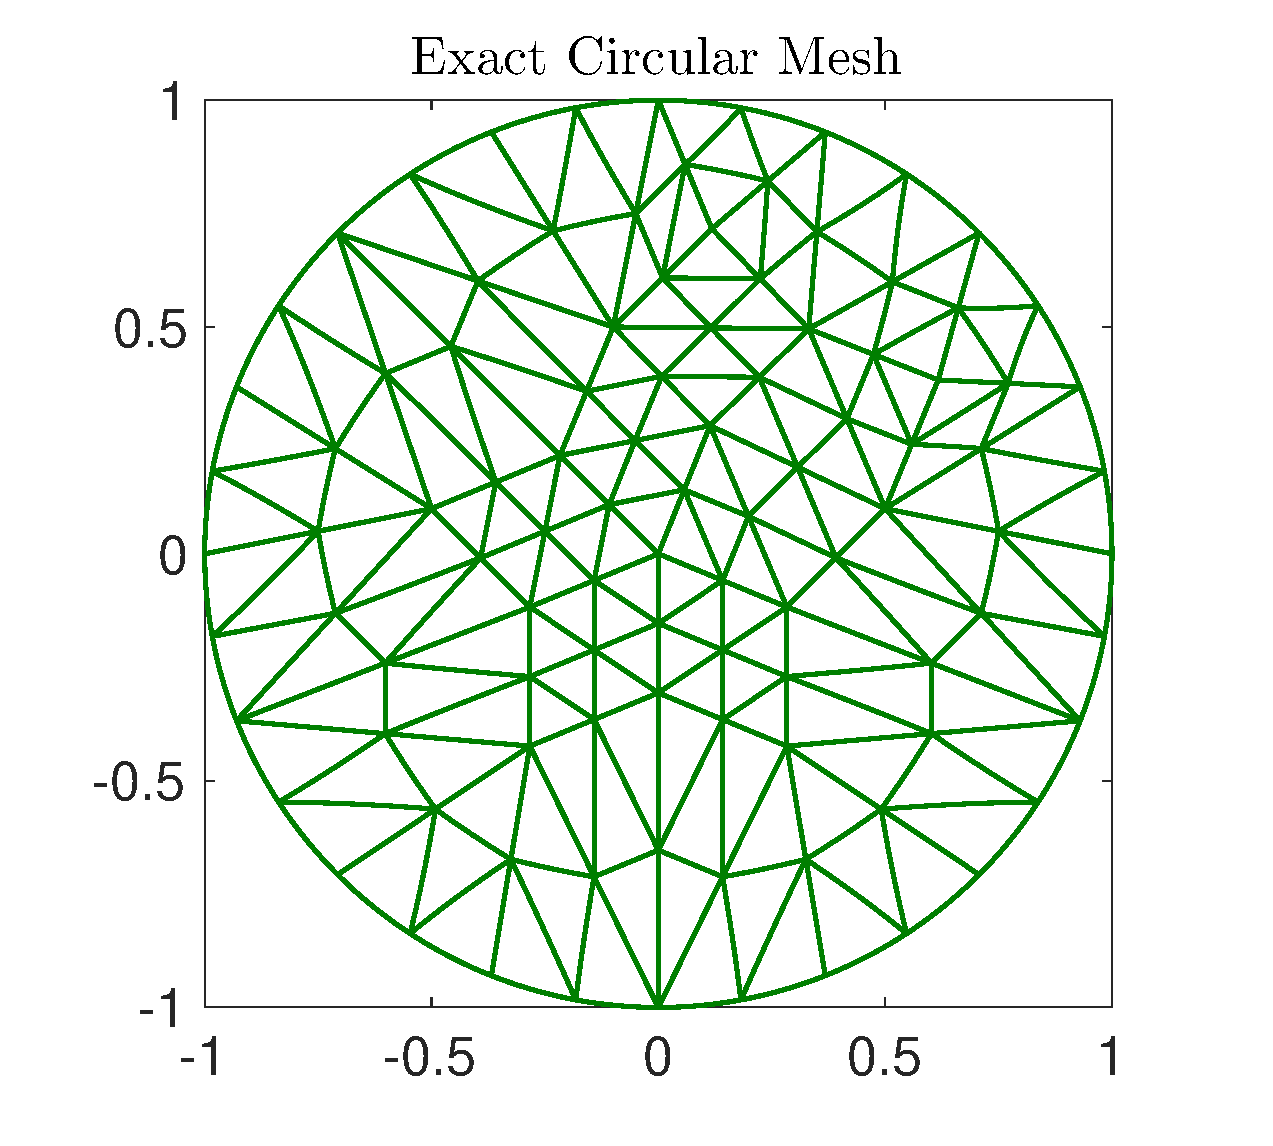
\includegraphics[width=0.8\linewidth]{./bidg_data/168_circ}
\end{center}
\vspace*{-.5cm}
\caption{Exact b\'{e}zier circular mesh used in the scaling study.}
\label{fig:dns_scaling}
\end{figure}


The discontinuous Galerkin method, on the other hand, excels in aspects of its computational efficiency in the context of modern architectures, particular in convection-dominated flows that allow for localization of finite element stencils in such a way that dynamic problems lead to block diagonal matrix systems.  The locality of the memory footprint in these application models leads to the ability to compute at high local order at unusally high arithmetic intensity cite.

The BIDG method merges these two methods seamlessly way cite, by utilizing an peicewise rational isogeometric basis for the geometric representation, a peicewise discontinuous po9lynomial representation for the model, and an exact (and properly conditioned) geometric transformation between the two spaces.

For our scaling test here we solve the first-order acoustic wave equation: \begin{equation} \label{awe} \frac{\partial p}{\partial t} + \nabla\cdot \boldsymbol{u} = 0, \quad  \frac{\partial\boldsymbol{u}}{\partial t} + \nabla p = 0, \end{equation} where $\boldsymbol{u}=(u_x,u_y)$ is the velocity, and $p$ the pressure.

Broadly such a system is discretized by solving the semidiscrete system \[ \left( v, \frac{ \partial A}{\partial t} \right)_{\Omega_{i}}= V_{\Omega_{i}}+S_{\partial\Omega_{i}} \] for $A = (p,\boldsymbol{u})$, $V_{\Omega_{i}}$ a volume kernel that has only elementwise dependencies, and $S_{\partial\Omega_{i}}$ a surface kernel that depends on interelement communication through a classical upwinding flux cite.  


\begin{figure}[h]
\begin{center}
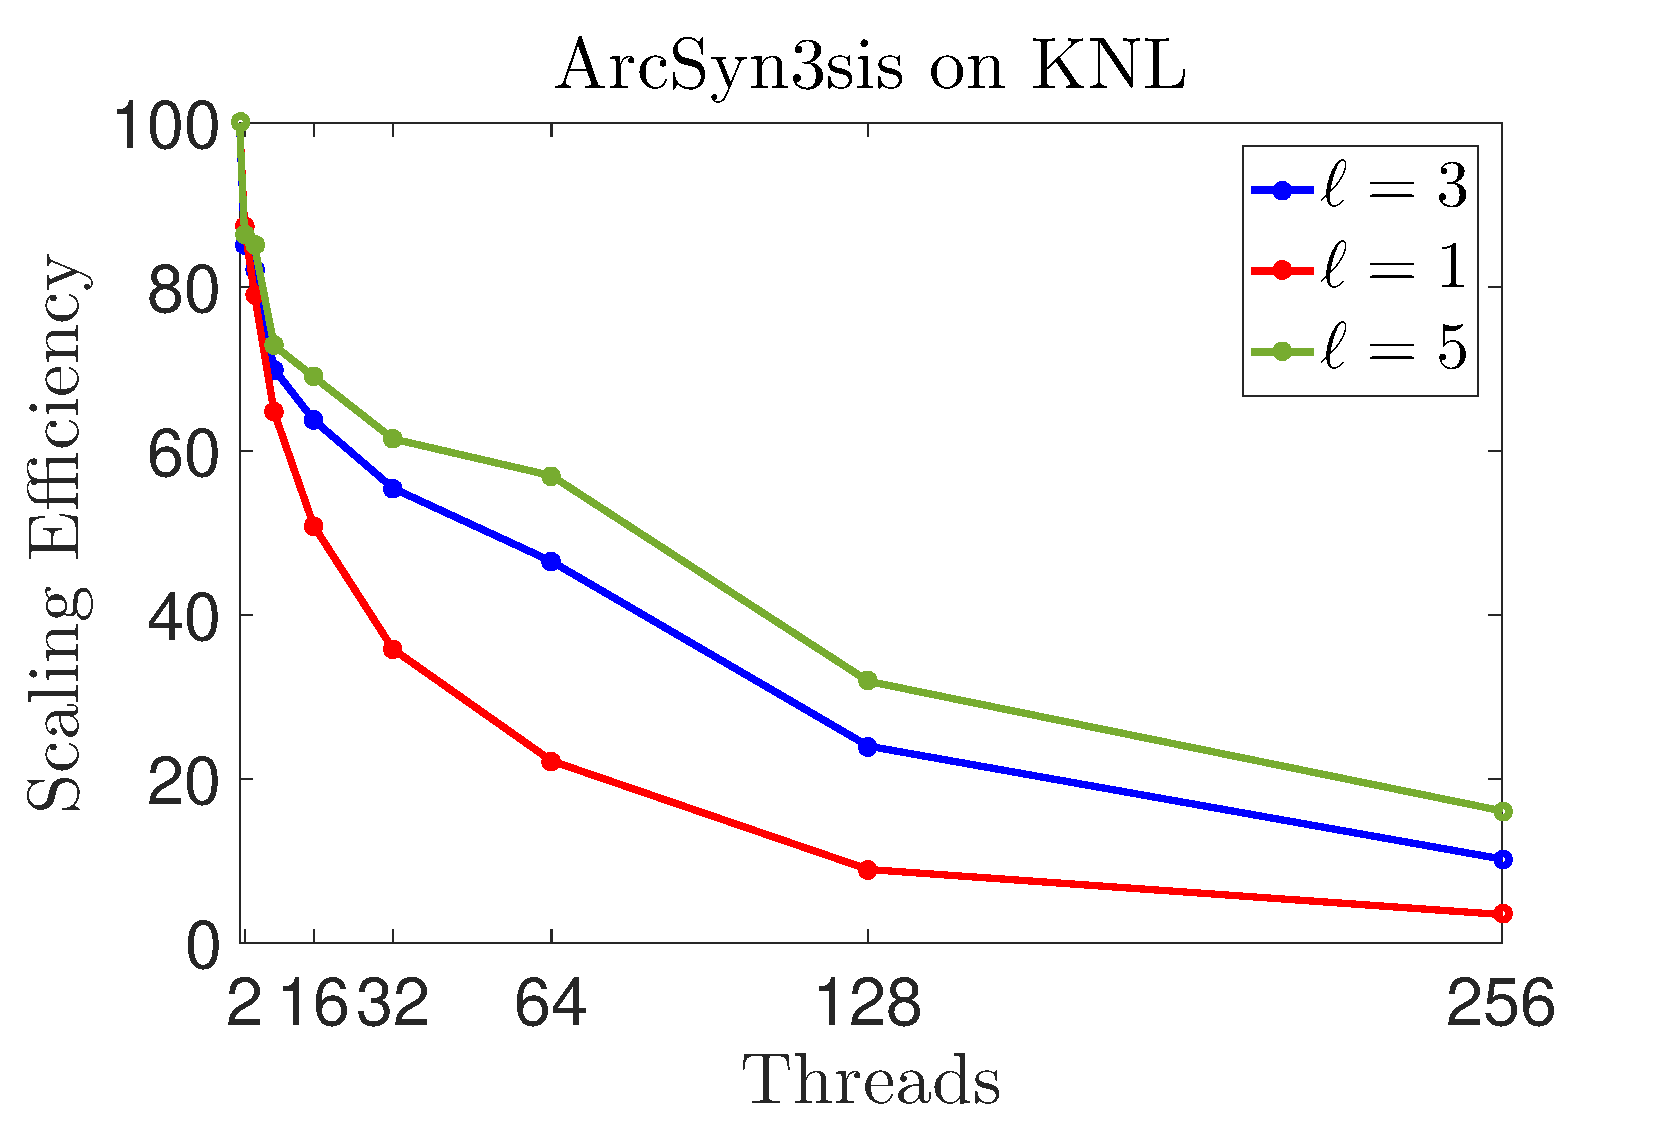
\includegraphics[width=0.95\linewidth]{./bidg_data/scaling_p}
\end{center}
\vspace*{-.5cm}
\caption{Strong scaling of ArcSyn3sis BIDG kernel on KNL nodes.  Test run on isogeometric mesh with 168 elements.}
\label{fig:dns_scaling}
\end{figure}


The implementartion on isogeometric meshes 


%
% NM --- feel free to disregard anything I recommend here
%
 %yar\todo{Discuss, broadly, what class of problems this resides in and why humanity works on it}

%% yar2\todo{some basic intro to the linear algebra you are doing}

%% yar3\todo{any nuances of porting to MIC?}

%% yar4\todo{discussion of scalability observed}

%% \missingfigure{Strong scaling of the GPs on a single MIC (e.g. problem size constant
%% and increasing number of threads)}

%Finally, some discussion is needed: is DG ameniable to MICs? Vs typical CPUs? I
%naively guess so, since you can essentially vectorize several of the
%activities.

